\documentclass[../notesdecours]{subfiles}

\begin{document}
\chapter{Principes fondamentaux de la physique quantique}\label{chap:chap2}

\section{Dualité onde-corpuscule de la lumière}
La lumière a toujours été dans l'histoire une source d'interrogation. Elle nous sert à voir littéralement, mais certaines manipulations avec permettent d'en étudier la nature. Corpuscule ? Ondulatoire ? Les deux hypothèses se combattaient au XVIIè siècle, avec Christophe Huygens qui défendait une théorie ondulatoire et Isaac Newton qui défendait une théorie corpusculaire. \\

Au XIXè siècle, des expériences de diffraction (phénomène purement ondulatoire) menées par Thomas Young et Augustin Fresnel ont permis d'affirmer que la lumière possédait des propriétés ondulatoires. Newton part donc avec un point en moins. Un siècle plus tard, Einstein émet une théorie corpusculaire de la lumière, certaines raisons l'ayant poussé à le faire. Parmi eux, les travaux de Planck. \\

Max \textsc{Planck} étudiait les corps noirs (enceinte macroscopique qui absorbe entièrement tout rayonnement incident, à l'équilibre thermodynamique entre la matière qui le constitue et son propre rayonnement -- voir PHYS-F201) et de ses études est ressorti un paramètre qui a les dimensions d'une énergie fois un temps (unités : $\mathrm{Js}$), appelé \textit{constante de Planck}. Ce paramètre qu'on note $h$ décrit formidablement les propriétés des corps noirs -- plus précisément, la densité d'énergie de rayonnement d'un corps noir (toujours, voir PHYS-F201). Le résultat obtenu par Planck n'était cependant pas en accord avec la mécanique classique. De son côté, Albert Einstein propose une théorie corpusculaire de la lumière, qui va en accord avec les résultats de Planck, en utilisant notamment cette même constante $h$ pour décrire \textbf{l'effet photoélectrique} \footnote{Effet expliquant l'émission d'électrons par un métal exposé à de la lumière dans certaines conditions.}. Ceci souligne l'importance de $h$ car le corps noir et le métal n'ont \textit{a priori} rien en commun. La constante de Planck est donc une des \textit{constantes fondamentales de l'Univers}.
$$h \approx 6.63 ; 10^{-34} \; \mathrm{Js}$$
Le caractère fondamental de la constante de Planck lui procure également un autre surnom : le \textit{quantum d'action}.


\subsubsection{Effet photoélectrique}
En bombardant une plaque métallique de lumière de longueur d'onde $\lambda$ (maintenant qu'on sait que la lumière est une onde), on remarque qu'au-delà d'une certaine fréquence seuil $\nu_0$ ($\lambda$ et $\nu$ sont liées par $\lambda = c/\nu$), des électrons sont émis avec une énergie qui augmente linéairement avec la fréquence, avec une pente de $h$, et dont l'expression de son énergie cinétique $T$ est donnée par :

$$ T = h\nu - W$$
où $W = h \nu_0 \equiv$ Travail d'extraction, autrement dit, c'est le travail que doit fournir l'électron pour s'extraire de la plaque métallique. Nous pouvons voir que ce travail correspond à une énergie de fréquence $\nu_0$, la fréquence seuil. 

\subsubsection{Les particules de lumière}
Einstein est amené à établir une relation entre la longueur d'onde de la lumière et une impulsion (à travers le nombre d'onde, ou plus précisément, le vecteur d'onde $\vec{k}$).
En effet, nous savons par le cours de relativité et électromagnétisme que l'énergie totale d'une particule est donnée par $E = m \gamma c^2$, tandis que l'impulsion vaut $\vec{p} = m \gamma \vec{v}$. Ainsi, nous avons la relation $\vec{p} = \frac{E}{c^2} \vec{v}$. 
Or si l'on considère bien la lumière comme une particule, nous pouvons exploiter ces relations. Sa vitesse étant de plus constante, de norme $c$, nous en déduisons que : 
\begin{align*}
  p &= \frac{E}{c^2} c = \frac{E}{c} = \frac{1}{c} \hbar \omega \\
  &= \hbar k 
\end{align*}
où nous avons employé la relation de dispersion pour la lumière $\omega = kc$. \\
Le fait que $E = pc$ nous donne, par $E^2 = m^2 c^4 + c^2 p^2$, que la particule qui décrit la lumière est de masse nulle. \\
En résumé, nous avons donc ces deux relations très importantes qui relient la lumière, une onde, à un caractère corpusculaire ; 
\begin{align}
\label{Quantification energie et impulsion}
\left\{ \begin{array}{l}
E \equiv \hbar \omega \quad \text{\small (quantification de l'énergie}) \\
\vec{p} \equiv \hbar \vec{k}  \quad \text{\small (lien longueur d'onde-impulsion)}
\end{array} \right.
\end{align}

L'introduction d'une particule de lumière, a.k.a le \textbf{photon} n'est pas super appréciée et nécessite donc d'être démontrée. C'est ce qu'a fait Arthur Compton expérimentalement. Il a démontré que lors d'une interaction (une collision) photon-électron, l'impulsion et l'énergie du photon étaient conservées, tout comme une particule classique. Le photon est donc bien une particule. Et c'est aussi une onde (\textit{cf.} franges de Young). 
\begin{center}
\begin{large}
\textit{La lumière se comporte donc à la fois comme une onde \underline{et} comme une particule.}
\end{large}
\end{center}

\subsection{Observation de la dualité onde-particule de la lumière}
On reprend l'expérience des fentes de Young et cette fois-ci en lumière atténuée, pour voir la figure d'interférence se construire progressivement. On alors les impacts un par un, \textbf{photon par photon} mais à long terme on voit se dessiner une figure d'interférence, cela veut dire que la lumière est une onde qui passe par les deux fentes à la fois.

\begin{itemize}
\item Nature corpusculaire : les impacts individuels.
\item Nature ondulatoire : la lumière passe par les deux fentes à la fois (figure d'interférence).
\item Dualité onde-particule : la lumière est à la fois partout et à un seul endroit. \end{itemize}

Une grande morale à cette section est que mine de rien, Einstein a développé et cru en une théorie qui allait à l'encontre de ce qui a été imaginé et prouvé par l'expérience depuis le siècle précédant, et ce malgré la splendide explication théorie de l'électromagnétisme de Maxwell, qui d'ailleurs ne laisse aucune invalidité dans son modèle prouvé par l'expérience ! Mais il y avait visiblement de la place pour une autre théorie. 

\section{Dualité onde-corpuscule de la matière}
L'aspect corpusculaire de la matière n'a pas besoin d'être introduit. En revanche, son aspect ondulatoire nourrit les interrogations rien qu'à l'usage de l'expression. C'est Louis de Broglie le véritable héros derrière cette hypothèse.

\subsection{Hypothèse de de Broglie}

Par la section précédente, nous avons compris que les travaux de Max Planck et d'Einstein permettent de dire qu'un rayonnement lumineux de fréquence $\nu$ est porteur d'énergie $E = h \nu$. \\
Durant la même époque de ces travaux, les spectres d'émission et d'absorption de certains atomes (notamment l'hydrogène) étaient étudiés, et la quantification de l'énergie absorbée par ces atomes permettait de bien expliquer le fait que l'on observait un spectre de raies fines distinctes. \\
En effet, on observa qu'un électron d'un atome ne peut passer d'un état à l'autre qu'en absorbant (ou émettant) une quantité bien définie d'énergie $E_{ij}$ : 
$$E_{ij} = h\nu_{ij} = |E_i - E_j|$$
où $E_i$ correspond à l'énergie d'un état $i$. \\

La mécanique classique ne permettant pas d'expliquer ce phénomène, Louis de Broglie a alors émis l'hypothèse 
\wrap{15}{r}{0.4}{\centering \vspace{-0.5cm}
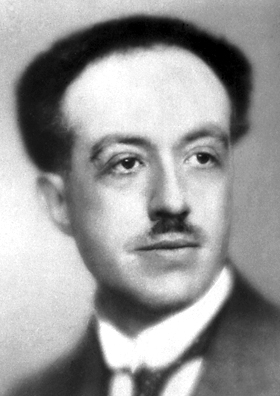
\includegraphics[width=0.6\linewidth]{images/Louis_de_Broglie}
\caption{Louis de Broglie. Il obtint le prix Nobel en 1929 à 37 ans pour la découverte de la nature ondulatoire de l'électron.}}
que \textbf{tous les corpuscules matériels peuvent avoir un aspect ondulatoire}, et que les aspects corpuscule et ondulatoire sont reliés par la formule \eqref{eq:debroglie}.
\begin{equation} \label{eq:debroglie}
\boxed{
\left\{ \begin{array}{ll}
E &= \hbar \omega \\
\vec p &= \hbar \vec k
\end{array} \right. \implies \lambda = \frac{h}{p} \quad \text{ \textit{(Relation de de Broglie)}}} 
\end{equation}

Son hypothèse a ensuite été validée lorsqu'il a réussi à montrer des figures d'interférences par diffraction d'électrons. \\
Les relations d'Einstein pour le photon se généralise donc pour des particules, à l'échelle microscopique (en effet, les aspects ondulatoires de la matières deviennent négligeables au niveau macroscopique). \\
Il faut bien comprendre l'étape à laquelle nous sommes ; c'est de la que se construit une nouvelle physique qui est la mécanique quantique. \\

Il faut dès lors commencer à prendre en compte, dans les équations, l'aspect ondulatoire d'une particule. Ce qui peut alors se faire est de décrire une particule par une équation d'onde (l'équation d'onde EM pour le photon).\\
La section suivante vise donc à montrer comment arriver à l'équation de Schrödinger, autrement dit, comment arriver à établir une relation qui décrit une particule quantique de manière ondulatoire. 

\subsection{Vers l'équation de Schrödinger}
Considérons un corpuscule matériel. \\
Nous allons lui associer une fonction d'onde qui est solution de l'équation d'onde ; ainsi, le corpuscule correspondra bien à la définition d'une onde. \\
En utilisant cette équation d'onde, nous allons en premier lieu \textbf{établir une équivalence} entre des grandeurs physiques et des opérateurs. \\
En deuxième lieu, il nous suffira de relier ces grandeurs physiques avec les relations \ref{Quantification energie et impulsion}, ainsi qu'avec l'expression de l'énergie d'une particule (donnée en électromagnétisme).
On obtiendra finalement une équation liant plusieurs aspects de la fonction d'onde.\\

\begin{enumerate}[label =  (\alph*)]
\item \textit{Équivalence entre opérateurs}. \\
L'équation d'onde est de la forme : 
$$\left(\dfrac{1}{c^2} \partial_t ^2 - \Delta \right) \vec A = 0$$
et une solution possible de cette équation est l'onde place, c'est-à-dire une fonction de la forme : $$
A(\vec{x}, t) = A_0 \; e^{-i(\omega t - \vec k \cdot \vec x)} \; .$$
De ce fait, nous pouvons en déduire que : 
\begin{itemize}
\item dériver $A$ par rapport au temps revient à multiplier $A$ par $-i\omega$,
\begin{equation}
\label{équivalence pulsation}
  \boxed{\omega \longleftrightarrow \dfrac{i}{A} \partial_t A} \; 
\end{equation}
\item prendre le gradient revient à multiplier par $i\vec k$, 
\begin{equation}
\label{equivalence nombre d'onde}
  \vec k \longleftrightarrow -\dfrac{i}{A} \vec \nabla A \quad \Rightarrow \quad \boxed{k^2 \longleftrightarrow -\dfrac{1}{A} \Delta A} \; 
\end{equation}
\end{itemize}

\item \textit{Recherche d'une relation à exploiter}. \\
Afin de décrire notre système quantique, nous allons utiliser une équation représentant son énergie, dans lequel nous pourrons exploiter les relations d'équivalence \ref{équivalence pulsation} et \ref{equivalence nombre d'onde} obtenues précédemment. 
De cette manière, nous aurons la représentation de l'énergie d'un système quantique, tout en ayant tenu compte de son caractère ondulatoire.\\

Plus particulièrement, relions donc d'abord la pulsation $\omega$ et le nombre d'onde $k$ avec l'énergie et l'impulsion, ce qui est possible grâce à \ref{Quantification energie et impulsion} ; ainsi, nous avons 
\begin{equation} \label{eq:ch2-correspondance}
  \left\{ \begin{array}{lll}
  E &= \hbar \omega &= \dfrac{i\hbar}{\psi} \partial_t \psi \\
  \vec p &= \hbar \vec k &= -\dfrac{i\hbar}{\psi} \vec \nabla \psi \Rightarrow p^2 = -\dfrac{\hbar ^2}{\psi} \Delta \psi
  \end{array} \right. \Longrightarrow \quad \boxed{\begin{array}{ll}
  E &=\dfrac{i\hbar}{\psi} \partial_t \psi \\
  p^2 &=  \dfrac{i\hbar}{\psi} \partial_t \psi
  \end{array}}
  \end{equation}
où $\psi$ est ce que l'on va appeler la fonction d'onde du système quantique. 
Ensuite, exploitons une relation qui fait intervenir les grandeurs $E$ et $p$. Nous allons y distinguer 2 cas :

\begin{enumerate}[label = \roman*)]
\item Cas relativiste : 
$$E^2 = m^2 c^4 + p^2 c^2$$
La substitution des relations de \eqref{eq:ch2-correspondance} dans cette relation décrit le comportement d'une particule quantique relativiste et constitue l'\textbf{équation de Klein-Gordon}.
\begin{equation} \label{eq:dirac}
\boxed{\text{Équation de Klein-Gordon} : \quad -\hbar ^2 \partial_t ^2 \phi + c^2 \hbar ^2 \Delta \phi - c^4 m^2 \phi = 0}
\end{equation}
De ce que l'on peut voir, elle est d'ordre 2 en le temps, autrement dit, sa non-linéarité rend la résolution de l'équation trop compliquée à notre niveau. Cette équation sera donc traitée en BA3.
\item Cas non-relativiste :
$$E = \dfrac{p^2}{2m} + V(\vec r, t)$$
De manière similaire, on obtient l'équation de \textbf{Schrödinger} :
\begin{equation} 
\boxed{\text{Équation de Schrödinger} : \quad
i\hbar \dfrac{\partial}{\partial t} \psi = -\dfrac{\hbar ^2}{2m} \Delta \psi + V(\vec r, t) \psi}
\end{equation}

\end{enumerate}
\end{enumerate}
En général, il ne sera pas possible de trouver des solutions analytiques, mais nous verrons plus tard qu'avec des approximations appropriées, il est possible
d'en tirer des conclusions intéressantes. Le cas non-relativiste d'une particule est d'ailleurs celui que nous allons étudier profondément cette année (en particulier, c'est le sujet de tout le chapitre suivant, où ses propriétés et son interprétation seront discutées, munis de quelques exemples).
Notons également que les solutions $\psi$ (fonction d'onde associée à une particule quantique) de cette équation de Schrödinger sont ce qui permettent de décrire l'état de la particule. Autrement dit, la fonction d'onde contient toutes les informations nécessaires sur la particule. 


\end{document}
